
\chapter{Introduccion}
\label{capitulo1}
\lhead{Capítulo 1. \emph{Introduccion}}
% De qué va a tratar el capítulo

La navegación y exploración en áreas de difícil acceso mediante el uso de robots, es una tarea que se ha venido desarrollando en el Grupo de Investigación y Desarrollo en Mecatrónica de la USB  \textit{(GIDM)} desde hace mu tiempo. Donde una de las aplicaciones mas demandantes, es la tarea de reconstruir un mapa 2D de la superficie mapeada por los robots utilizados. En el presente capitulo se pretende introducir los trabajos previos y avances que se han tenido en el desarrollo de este tipo aplicaciones, tanto en el \textit{GIDM} como a nivel mundial, y que dieron origen y motivación para la realización del proyecto. Además, de postular un serie de problemas que el presente trabajo busca solucionar.

\section{Antecedentes}

Cuando hablamos de construir un mosaico 2D, se hace referencia al proceso de recortar y alinear imágenes, de tal forma que puedan ser representadas todas juntas en una sola gran imagen. Partiendo de que estas imágenes sean tomadas desde diferentes ubicaciones de la cámara, a diferencia del proceso para elaborar imágenes panorámicas, en las cuales esta ubicación es una constante. 

La elaboración de mosaicos para la construcción de mapas del suelo, se ha desarrollado incluso antes desde la era digital de la computadoras. Desde que el proceso de registrar fotografías ha existido, se comenzaron a usar para elaborar mapas topográficos \cite{primeros-mapas}, donde imágenes adquiridas a partir de globos aerostáticos o altas colinas eran unidas manualmente. Posteriormente, producto de los avances en la creación de aviones, el interés por la aerofotografía se incrementó en gran medida. Pero debido a que no se alcanzaban grandes altitudes, y a la continua necesidad de mapear grandes áreas, era necesario que los mapas se construyan mediante fotografías que se superpongan, de igual forma esta tarea se llevaba a cabo mediante técnicas manuales por medio de expertos.

La necesidad de registrar áreas aun mas grandes siguió avanzando, motivado por la llegada de los satélites que eran capaces de enviar a tierra la información que obtenían de las cámaras. Los avances tecnológicos en materia de computación, y el creciente aumento de datos por para esta aplicación, promovieron el desarrollo de técnicas de procesamiento de imágenes para dar solución a este tipo de problemas.

Del mismo modo, distintos centros de investigación en el área de la física, robótica y visión por computadora, han aplicados sus esfuerzos al algoritmos para la realización de estos mapas en ambientes mas desafiantes como lo son el fondo marino \cite{gracias-victor,Pizarro-singh,eustice,Allais}. Cuando se opera en este tipo de ambientes, en busca de realizar exploraciones mas eficientes y a mayor escala, se emplean vehículos operados remotamente \textit{ROV} (del inglés: Remotely Operated Vehicles) o vehículos autónomos submarinos \textit{AUV} (del inglés: Automated Underwater Vehicles). 

En el \textit{GIDM} se han realizado grandes avances en el desarrollo de equipos y plataformas robóticas, específicamente para su uso en aplicaciones submarinas. En este sentido, se cuenta con un vehiculo sumbarino llamado OpenROV\footnote{\url{hugin.sourceforge.net/}}

\begin{wrapfigure}{r}{0.3\textwidth}
	\begin{center}
		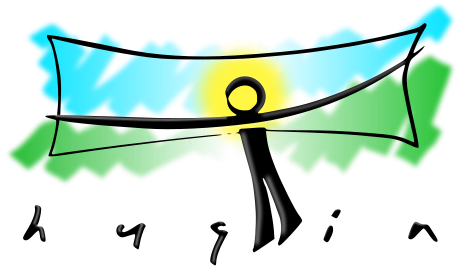
\includegraphics[width=0.3\textwidth]{hugin}
	\end{center}
	\caption{Logo del software Hugin}
\end{wrapfigure}

En el \textit{GIDM} actualmente se utilizan mecanismos manuales para la elaboración de estos mapas, en especifico, se hace uso de \textit{softwares} como Hugin\footnote{\url{hugin.sourceforge.net/}}. Este es un programa de código abierto y gratuito bajo licencia GPL\footnote{\url{http://www.gnu.org/copyleft/gpl.html}}, el cual esta dedicado a la generación de imágenes panorámicas, incluyendo funciones para el recorte, alineación, corrección de color; además de algoritmos para la optimización de parámetros en la cámara, y corrección de distorsión. Si bien este software esta diseñado para la creación de imágenes panorámicas, permite el uso de varios tipos de proyecciones cartográficas, entre estas la rectangular, proyectando las imágenes sobre un plano recto.

 

\section{Justificación y planteamiento del problema}

Para esta tarea, es común el uso de herramientas que requieren de una gran intervención por medio del usuario para la elaboración de un mapa.
    
Atendiendo a esta necesidad, es necesario contar con un sistema que permita realizar la reconstrucción del suelo con la menor interacción posible del ser humano. Asimismo, con el fin de poder realizar operaciones de mapeo y localización simultanea \textit{SLAM}, haciendo uso de las herramientas y robots existentes en el laboratorio, es necesario contar con un sistema basado en visión, que genere de forma automática un mapa 2D de la superficie sobre la que navega o sobrevuela el vehículo remoto.


\section{Objetivos}

\subsection{Objetivo General}

Analizar e implementar un sistema automatizado que permita la reconstruccion de un mapa en dos dimensiones, del entorno recorrido por robot, aereo o submarino.

\subsection{Objetivos Específicos}

\begin{itemize}
	\item Análisis comparativo de metodos vigentes en la reconstruccion de mosaicos 2D, a partir de imagenes y videos de entrada.
	\item Implementacion de modulo de preprocesamiento y correccion de entrada.
	\item Analisis comparativo de metodos de deteccion y description de puntos clave.
	\item Implementación de módulo de alineación de imagenes mediante la deteción de puntos clave.
	\item Cuantificar el error de reproyeccion y distorsion en los modelos 2D generados.
\end{itemize}

\section{Estructura del trabajo}

Luego de presentar el planteamiento del problema y la descripción del proyecto, la presente investigación se encuentra dividida en 5 capítulos, organizados de la siguiente manera:

En el \textit{\textbf{Capitulo 2}} se presenta una revisión del estado del arte, en el cual se exponen los distintos métodos para la detección e identificación de puntos de interés en una imagen. Además, se presentan diversos algoritmos utilizados en la actualidad para la alineación de imágenes en un mosaico. Finalmente, se muestran las técnicas que se utilizan para la fusión entre las imágenes, que logran reducir errores en el color, y la calidad del mapa final.

El \textit{\textbf{Capitulo 3}} describe cada cada uno de los módulos necesarios en la construcción del mosaico, así como también una descripción detallada de los algoritmos implementados.

Los resultados experimentales son mostrados en el \textit{\textbf{Capitulo 5}}, en este se contemplan los modelos generados de forma automática del suelo, tanto terrestre como submarino. Además se presenta un análisis comparativo de estos resultados sobre los que proveen herramientas no automatizadas.

Finalmente, en el \textit{\textbf{Capitulo 6}} se presentan las conclusiones que se derivaron del proyecto, por otra parte, se plantean trabajos futuros que podrían dar pie a posibles mejoras en la linea de investigación del presente trabajo.